%******************************************************************************
% Theory
%******************************************************************************
\chapter{Theory}\label{ch:theory}


\section{Java}\label{sec:java}
Java is one of the most popular programming language.
It is developed by Oracle Corporation on May 23, 1995.
It is also used to develop mobile apps, web apps, desktop apps, games and much more.
It has helped to reduce costs, shortens development timeframes, drive innovation,
and improve application services.
\medskip

\noindent
There are five primary goals in the creation of the Java language.
\begin{itemize}
    \item It must be simple, object-oriented, and familiar.
    \item It must be robust and secure.
    \item It must be architecture-neutral and portable.
    \item It must be interpreted, threaded and dynamic.
\end{itemize}


\section{Socket}\label{sec:socket}
Socket programming in Java provides a tool that allows communication between two applications
that run on different devices.
Socket allows a connection between a client and a server.
Typically, it provides a way to connect two nodes on a network to exchange data.
One node listens on a specific port on an IP, while the other socket connects to the other to
establish a stable connection.
\medskip

\noindent
Initially, the client must wait for the server to start.
While the server is running, the client must send a request to the server and wait for its
response.
The socket connection uses two computers that have the necessary information about each
other's location on the network location, i.e.IP address and port.


\section{Thread}\label{sec:thread}
A thread of execution is the smallest sequence of programmed instructions that can be managed
independently by a scheduler, which is typically a part of the operating system.
The implementation of threads and processes differs between operating systems,but in most cases
a thread is a component of a process.
The multiple threads of a given process may be executed concurrently
\(via multithreading capabilities\), sharing resources such as memory, while different
processes do not share these resources.
\medskip

\noindent
A thread is a thread of execution in a program.
The Java Virtual Machine allows an application to have multiple threads of execution running
concurrently.
Every thread has a priority.
Threads with higher priority are executed in preference to threads with lower priority.


\section{Git}\label{sec:git}
Git is an open source distributed version control system, mainly used for source code
management, with an emphasis on speed.
Git was initially designed and created by Linus Torvalds for Linux kernel development.
Git operates on a decentralized architecture, so every Git working directory is a
full-fledged repository with a complete history and full revision-tracking capabilities,
and is not dependent upon network access or a central server.
Unlike popular non-distributed predecessors, such as Subversion and CVS, Git only needs a
central server for one thing: publishing changes to users of that server.
You can equally share changes directly with other people without the need to consult a central hub.

%
%\section{Project}\label{sec:project}
%A project is well-defined task, which is a collection of several operations done in order to
%achieve a goal \(for example, software development and delivery\).
%\medskip
%\noindent
%A Project can be characterized as:
%\begin{itemize}
%    \item Every project may has a unique and distinct goal.
%    \item Project is not routine activity or day-to-day operations.
%    \item Project comes with a start time and end time.
%    \item Project ends when its goal is achieved hence it is a temporary phase in the lifetime
%    of an organization.
%    \item Project needs adequate resources in terms of time, manpower, finance, material and
%    knowledge-bank.
%\end{itemize}
%
%A software Project is the complete procedure of software development from requirement gathering
%to testing and maintenance, carried out according to the execution methodologies,
%in a specified period of time to achieve intended software product.


\section{Our Software Project}\label{sec:our-software-project}
In our project, we have developed an application where two or more users can interact and
exchange messages of different file types such as text, image, video, PDF, and so on.
Mainly there are two GUI windows which make the communication user-friendly and easy to
communicate.
First window is the server and the other is the client.
The server window has the main privilege of starting and stopping the application.
When the server is started, the clients can exchange messages.
The client sends a message to the server and the message is forwarded by the server to the
target user.
The recipient client can receive the message.
If necessary, admin can delete the clients or the group by selecting.
\medskip

\noindent
On the Client window, user can send messages to different users and groups.
First, user needs to select user or group he/she want to chat with other user or group,
user will be able to send text to the other user and group in the prototype version of our
application.There is small text area where user will be able to write in it and if they want
to attach other document with it,can add with add File button and forward it to other with send
button.
User can navigate other users and group using the search.
User can also select new contacts and create new group with users.
On the config tab, the ip address, port number and name of server and client can be seen and
can be saved if save button is clicked.
\medskip

\noindent
Our team divided the development of this application into different versions, with each new
version our team will add more functionality, features, try to fix bugs and provide
user-friendly experience to the users.In the version 1.0, users can simply chat with other user
and groups.
In the version 2.0, users will be able to send images,text files,pdf files etc.
In the version 3.0, user can send videos and play it on message window.
Later, our team will come with more ideas and work with user's suggestions to improve our
application.
\medskip

\noindent


\section{UDP Protocol}\label{sec:udp protocol}
UDP is a communication protocol implemented across the internet for especially time-sensitive
transmissions such as video playback or DNS lookups.
UDP provides a quick transfer of data.
Unlikely, as any other protocol it is also a way of transferring data between two computers in
network.
By UDP, data are sent in packets directly to the target IP address and port number,
without establishing a connection first.
One computer can simply start transferring data to others.
If there is any errors, loss, and duplication, the UDP doesn't resend the data.


\section{Our Protocol Segment Format}\label{sec:our protocol}
Our basic protocol segment consist of opcode, sender and receiver.
The bases are divided into different bytes arrays.
The first 4-bytes of protocol segment is reserved for opcode which whose basic functionality is
to store functionality like register,deregister, search, poller, message, create group, join group,
leave group and group message.
The second chunk of 16 bytes presents IP address of the sender computer.
The third chunk of 16 bytes reserved for the receiver IP Address.

\subsection{Register}\label{subsec:register}
To register the client with the server, the client must send the basic protocol, host name, and
port number to the server.
The 0x01 opcode is required to register a client with the server using this protocol.
The hostname requires 16 bytes of data to be stored as part of the protocol and the port number
requires 4 bytes of data.

\begin{figure}[htb!]
    \centering
    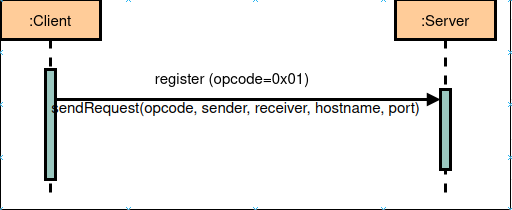
\includegraphics[width=0.7\textwidth]{gfx/protocoll_register}
    \caption{Register Client}
    \label{fig:register-client}
\end{figure}

\subsection{Deregister}\label{subsec:deregister}
To deregister, the client needs to send the opcode 0x02 to server with the sender and recipient
IP address.
Then the server logs off the client.

\begin{figure}[htb!]
    \centering
    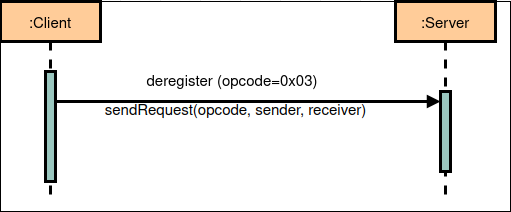
\includegraphics[width=0.7\textwidth]{gfx/protocoll_deregister}
    \caption{Deregister Client}
    \label{fig:deregister-client}
\end{figure}

\subsection{Search Clients}\label{subsec:search}
In order to get list of clients, client actually need to send the opcode 0x03 to the server.
After receiving this opcode, client get the all of all client on the server and will be able to
send message to the different client.

\begin{figure}[htb!]
    \centering
    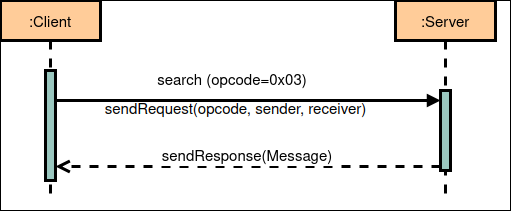
\includegraphics[width=0.6\textwidth]{gfx/protocoll_search}
    \caption{Get list of clients}
    \label{fig:client-list}
\end{figure}

\subsection{Puller}\label{subsec:poller}
Puller is actually send a signal to server.
If any new message is received by the server.
If server has received new messages, then it will return messages to client.

\begin{figure}[htb!]
    \centering
    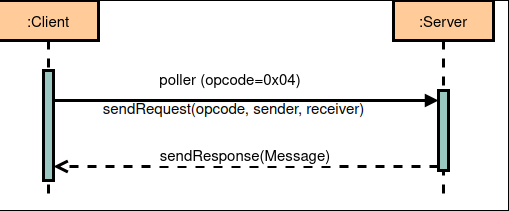
\includegraphics[width=0.6\textwidth]{gfx/protocoll_poller}
    \caption{Pull message}
    \label{fig:pull-message}
\end{figure}

\subsection{Message}\label{subsec:message}
If the sender wants to send data to the receiver, it must specify the base protocol and type
the content and the content itself, where the type of data is stored in 4 data bytes and the
content can have any length.
\medskip

\noindent
The type of data has five different type.
\begin{itemize}
    \item Message type register is presented by 0x01.
    \item Message type deregister is given by 0x02.
    \item Message type search is reserved as 0x03.
    \item Message type message and file is given by 0x04 and 0x05 respectively.
\end{itemize}

\begin{figure}[htb!]
    \centering
    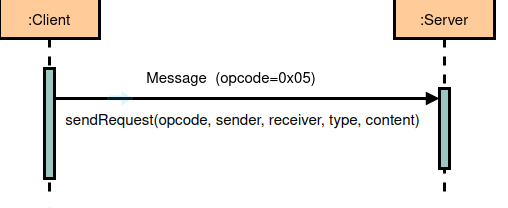
\includegraphics[width=0.7\textwidth]{gfx/protocoll_message}
    \caption{Send Message}
    \label{fig:send--message}
\end{figure}

\subsection{Create Group}\label{subsec:create}
To obtain a list of clients, the sender must use the opcode 0x03 with the IP address of the sender
and the recipient and the name of the group.
To create a group, sender needs to implement base protocol with 0x06 opcode and name of the group.
Usually, the hostname and name of group takes 16 bytes of data.

\begin{figure}[htb!]
    \centering
    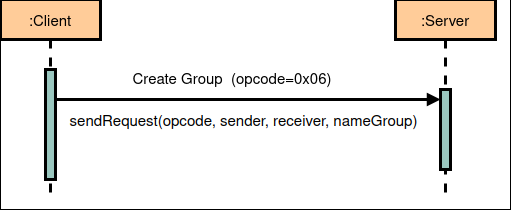
\includegraphics[width=0.7\textwidth]{gfx/protocoll_create_group}
    \caption{Create Group}
    \label{fig:group-create}
\end{figure}

\subsection{Join Group}\label{subsec:join}
In the same way, sender can to apply base protocol with 0x07 opcode and name of the group to join
the group.

\begin{figure}[htb!]
    \centering
    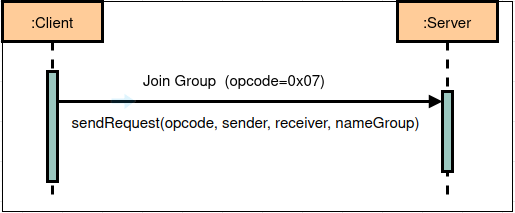
\includegraphics[width=0.7\textwidth]{gfx/protocoll_join_group}
    \caption{Join Group}
    \label{fig:join-group}
\end{figure}

\subsection{Leave Group}\label{subsec:leave}
By just changing opcode of above line to 0x08, sender can easily leave the group.

\begin{figure}[htb!]
    \centering
    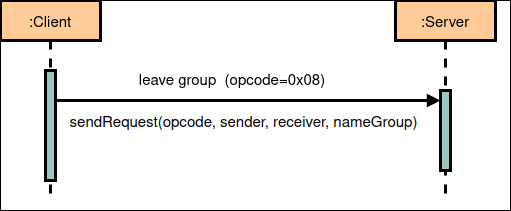
\includegraphics[width=0.7\textwidth]{gfx/protocoll_leave_group}
    \caption{Leave Group}
    \label{fig:leave-group}
\end{figure}

\subsection{Send Message to group}\label{subsec:send-message-to-group}
To send a message to a group, the sender who wants to send data to the group must specify the basic
protocol with opcode 0x09, in the addition of the name of the group of 16 bytes of data and the
type of the content and the content itself, where the data type is stored in 4 data bytes and where
the content can be of any length.

\begin{figure}[htb!]
    \centering
    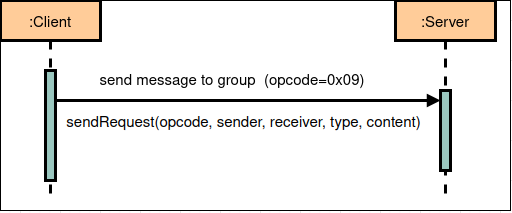
\includegraphics[width=0.7\textwidth]{gfx/protocoll_message_group}
    \caption{Send Message to group}
    \label{fig:send-message-to-group}
\end{figure}


\section{Improvement in Application}\label{sec:improvement-in-application}

\subsection{API-implementation}\label{subsec:apiimplementation}
To further improve our application in the future, we would use an API for frontend, backend and
database and to separate frontend, backend and database from each other.

\subsection{Usable on multiple devices} \label{subsec:usableonmultipledevices}
The current version of our application can be used on Linux, Mac and Windows.
In the upcoming version we will bring it to other devices like Android, tablets, etc.

\subsection{Implementation of database}\label{subsec:implementationdatabase}
Our team will integrate this application to store data, backup client and server data and
reimplementation of the data.

\subsection{Implementation on higher protocol}\label{subsec:implementation-on-higher-protocol}
To use it on a higher protocol, our team will apply it with the https protocol.
so we can use it in websites and browsers.

\subsection{Overall validation}\label{subsec:overall-validation}
To improve the viability of our application, we will add some validation features
to make the application more realistic and error-free.
And know that users are getting the right data.

\subsection{Validation of port number}\label{subsec:validation-of-port-number}
We would add some functions to confirm and validate the port number on the devices
that the data is transferred to the right person and device.


%   Reference
%    https://en.wikipedia.org/wiki/Java_(programming_language)%   https://www.oracle.com/java/
%    https://www.w3schools.com/java/
%    https://en.wikipedia.org/wiki/Thread_(computing)
%    https://en.wikibooks.org/wiki/Git
%    https://www.tutorialspoint.com/software_engineering/software_project_management.htm

